\documentclass[12pt,a4paper]{article}
\usepackage[utf8]{inputenc}
\usepackage{amsmath}
\usepackage{color}
\usepackage[colorlinks=true,linkcolor=black,urlcolor=blue]{hyperref}
\usepackage{amsfonts}
\usepackage{amssymb}
\usepackage{listings}
\usepackage{xcolor}
\usepackage{graphicx}
\usepackage{float}
\usepackage{enumitem}
\usepackage[left=2cm, right=2cm, top=2cm, bottom=2cm]{geometry}

\lstset{language=Python, breaklines=true}

\begin{document}

\begin{titlepage}
	\begin{center}
		\vspace*{1cm}
		\Huge
		\textbf{MM2090}
		
		\vspace{0.5cm}
		\Large
		\textbf{Final Assignment}
            
		\vspace{1.5cm}
		\textbf{Author}\\
		\vspace{0.25cm}
		\large
		\textsf{Archish S}\\
		\vspace{0.2cm}
		\normalsize
		\texttt{me20b032@smail.iitm.ac.in} \\
		Batch 7
		\\
		
		\vfill
       
		This is the submission file for \\
		\Large       
		End Semester Assignment 
        
        \normalsize    
		\vspace{0.8cm}
           
		Indian Institute Of Technology Madras\\
		\today
            
	\end{center}
\end{titlepage}

\tableofcontents
\newpage

\section{Question 1}

\subsection{Task}
Generate 10 random numbers $y_i$ between -1 and +1. Use these as points $\left(x_i,y_i\right)$ where $x_i=i$ and show them as a scatter plot. Fit a higher order polynomial over these points to generate a pattern of how a random noise would look like. Sample the polynomial to generate about 100 points in the interval $x_1$ to $x_{10}$. Superpose a plot of this data along with original points $\left(x_i,y_i\right)$.  Identify the peaks (location and height) programmatically. Print them out and confirm those with the plot.

\subsection{Solution}

Link to the GitHub repository for this question: \href{https://github.com/Xerefic/MM2090-Solutions/tree/master/Final_Assignment/question_1}{GitHub} \footnote{Repo: \url{https://github.com/Xerefic/MM2090-Solutions/tree/master/Final_Assignment/question_1}}

\subsubsection{Approach}
I used the scikit-learn\footnote{Source: \url{https://scikit-learn.org/stable/}} library to generate a polynomial of degree $n$ and used linear regression to fit the polynomial to the given data. Although this polynomial over fits the given data, it is fine as it retains the randomness of generated coordinates. \\
To find the extrema, I am traversing through the sampled polynomial and identifying the locations where the polynomial attains local maxima or minima. 

\subsubsection{Requirements}
Language of choice: python
\begin{lstlisting}[language=bash]
	pip3 install numpy
	pip3 install matplotlib
	pip3 install sklearn
	pip3 install scipy
\end{lstlisting}

\subsubsection{Output}


\paragraph{Locations of Extremas}

\begin{description}
	\item Maxima at x = 1.4084308430843084 and y = 2.195104229252479
	\item Minima at x = 3.164766476647665 and y = -0.7656559740882756
	\item Maxima at x = 5.218071807180718 and y = -0.19116876616108414
	\item Minima at x = 7.025372537253725 and y = -0.5251533421000687
	\item Maxima at x = 8.292639263926393 and y = -0.2132152812141186
	\item Minima at x = 9.61087108710871 and y = -1.7288452082816121
\end{description}


\subsubsection{Images}

\begin{figure}[!ht]
	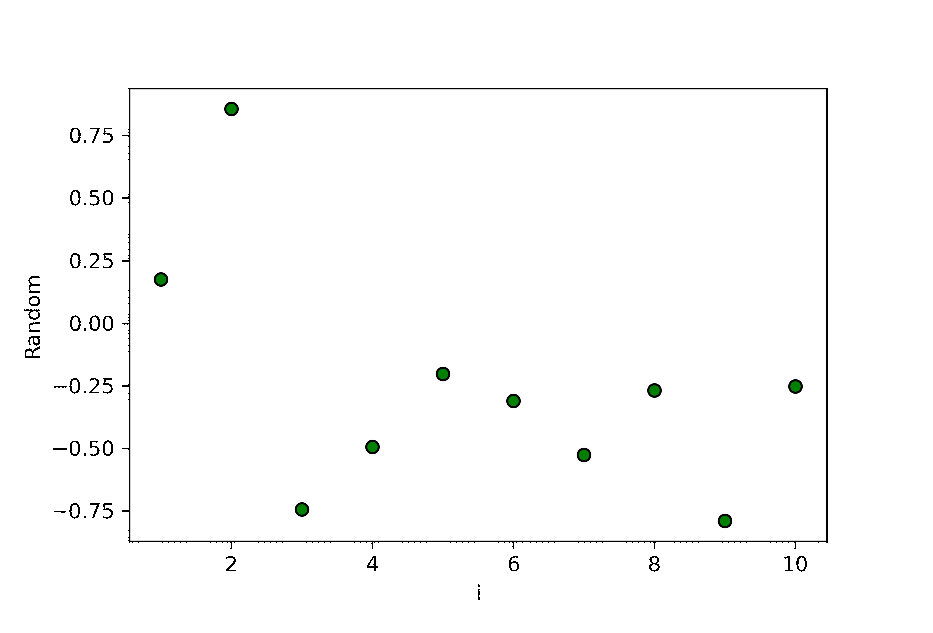
\includegraphics{question_1/Points.eps} 
	\caption{Generated Points}
\end{figure} 

\begin{figure}[!ht]
	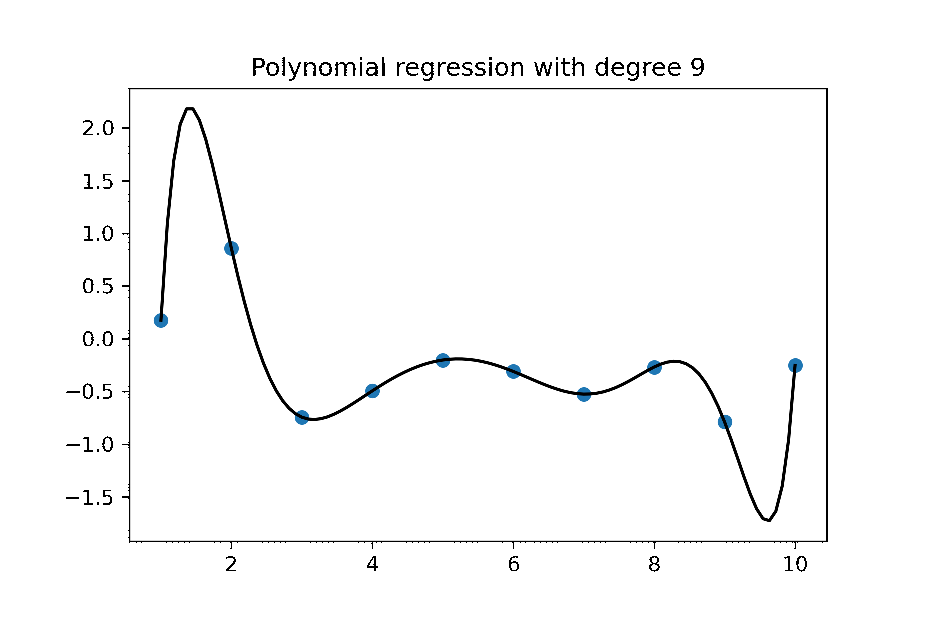
\includegraphics{question_1/Fitted.eps} 
	\caption{Fitted with Polynomial}
\end{figure} 

\clearpage
\subsection{Code}
\lstinputlisting{question_1/question1.py}
\clearpage
\section{Question 2}

\subsection{Task}
Consider the following sample images. Visually you can count that the number of objects in the images are 3, 2 and 5, respectively. Write a program that can take these images as inputs and report the number of objects as output. Assume that the objects are colored uniformly but different from the background which is also uniform. Do not assume the objects to be of same size or shape.
\begin{figure}[!ht]
\begin{center}
	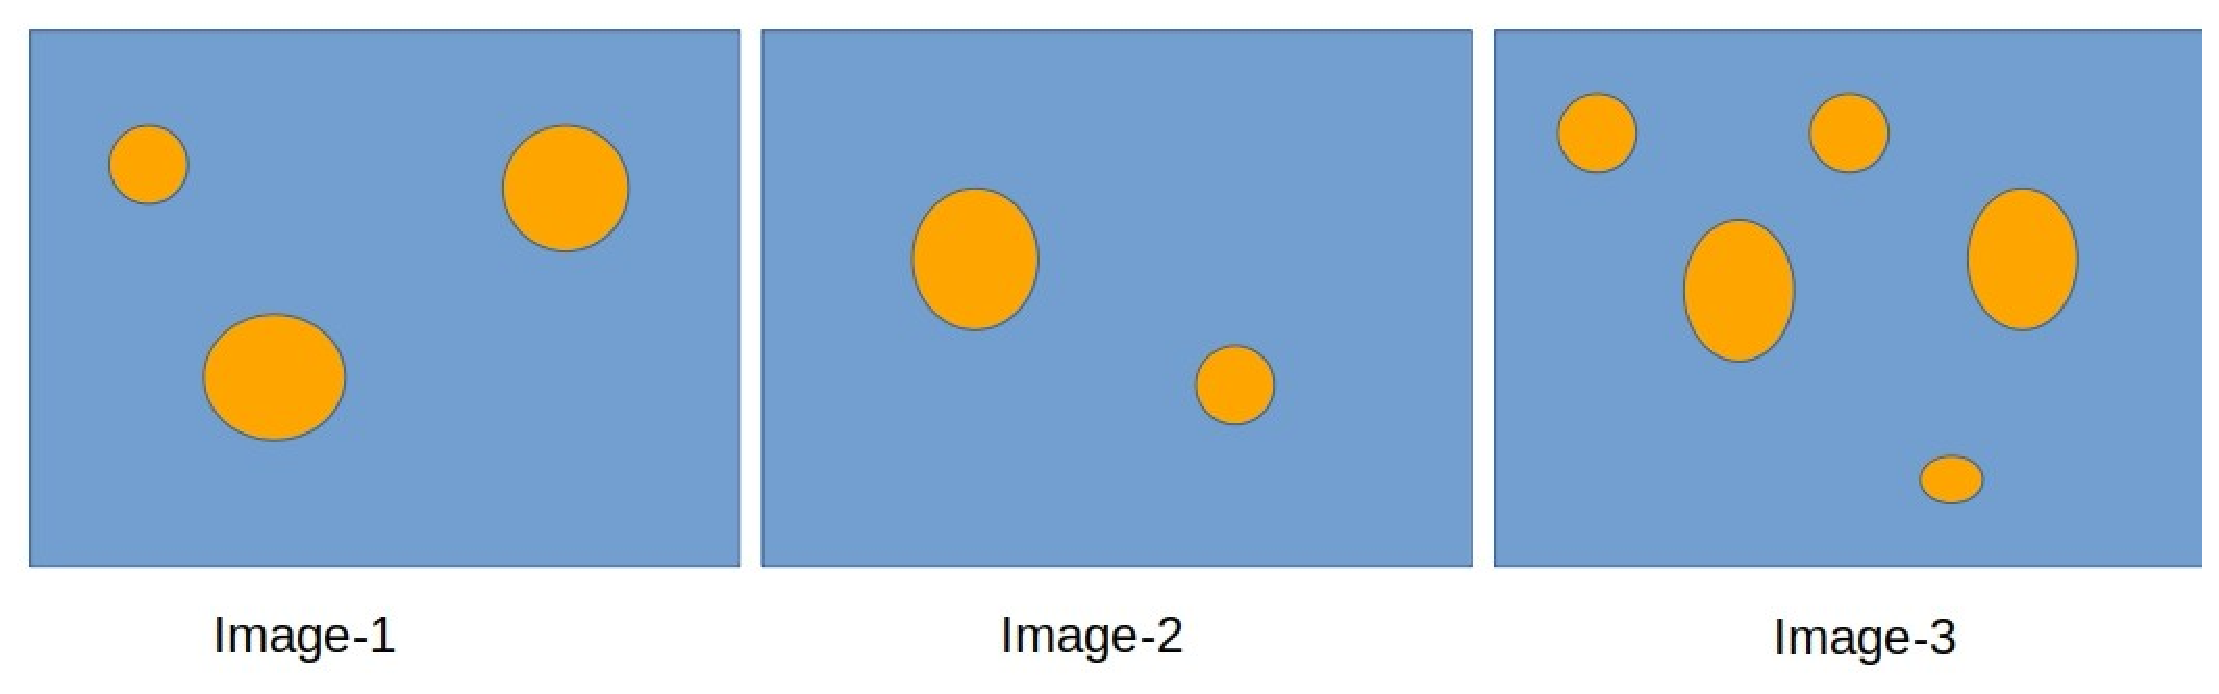
\includegraphics[width=0.75\paperwidth]{question_2/question2.eps} 
\end{center}
\end{figure} 


\subsection{Solution}

Link to the GitHub repository for this question: \href{https://github.com/Xerefic/MM2090-Solutions/tree/master/Final_Assignment/question_2}{GitHub} \footnote{Repo: \url{https://github.com/Xerefic/MM2090-Solutions/tree/master/Final_Assignment/question_2}}

\subsubsection{Approach}
I am using the OpenCV\footnote{Source: \url{https://opencv.org/}} library to pre-process the image – converting it to grayscale, and resizing for uniformity. Followed by applying a binary filter to sort the different colours into just two values – 0 and 255. Basically, every value greater than the minimum pixel value +10 is mapped to 255 and the rest to 0. Given that the image contains only two colours, this process will distinguish the two colours in every case. \\
To count the number of objects, I am using the fact that the gradients across the normal to the contours of the said region is non zero and uniform. findContours identifies continuous boundaries of regions having same colour, where the length of countours gives the number of the objects.


\subsubsection{Requirements}
Language of choice: python
\begin{lstlisting}[language=bash]
	pip3 install numpy	
	pip3 install matplotlib
	pip3 install opencv-python
\end{lstlisting}

\subsubsection{Output}

\begin{table}[!ht]
	\begin{center}
		\begin{tabular}{ | c | p{5cm} | }
			\hline
			IMAGE & PREDICTION \\ \hline
			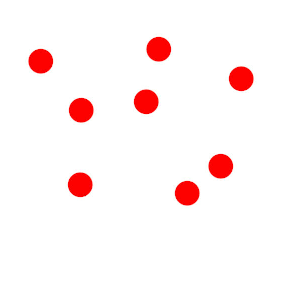
\includegraphics[width=50mm, height=50mm]{question_2/Image-1.eps} & 
				Number of objects = 8 \\ \hline
			
\includegraphics[width=50mm, height=50mm]{question_2/Image-2.eps} &
				Number of objects = 6 \\ \hline
		\end{tabular}
	\end{center}
\caption{Predicted Number of Objects}
\end{table}

\clearpage
\subsection{Code}
\lstinputlisting{question_2/question2.py}
\clearpage
\section{Question 3}

\subsection{Task}
Consider a temperature sensor placed near a valuable asset in a highly secure space. It records the local temperature every 5 seconds and writes it to a stream. The temperature data is flushed such that it keeps the data of only one hour. That is, you can view a window of only 720 data points at a time. Each new data point entering the window flushes the oldest data point out. Write two programs that do the following tasks.
\begin{itemize}
	\item Program-A when executed will continuously send temperature data that looks almost flat (say, room temperature with a small random noise within 0.5 Kelvin). This is to simulate the data coming from the temperature sensor. At predetermined instance, introduce a spike (sudden increase of temperature by 10 K) for 10 seconds and revert back to room temperature. This spike is caused due to the presence of an intruder.
	\item Program-B keeps reading the incoming data, detects the spike and reports the instance when it took place. Verify if the detection is accurate.
\end{itemize}
Think of the output from Program-A being piped to Program-B to perform this check. The stderr from both the programs about the spike should match. The stdout of Program-A contains the temperature data. You should submit a report on how this is made along with the two codes.


\clearpage
\section{Question 4}

\subsection{Task}
Simulate the Langton’s ant. Look up Wikipedia about what this problem is. Make sure you provide the formulation, program implementation and sample images to verify the behavior of the ant motion in the box. Consider a box of size $64*64$ for


\subsection{Solution}

Link to the GitHub repository for this question: \href{https://github.com/Xerefic/MM2090-Solutions/tree/master/Final_Assignment/question_4}{GitHub} \footnote{Repo: \url{https://github.com/Xerefic/MM2090-Solutions/tree/master/Final_Assignment/question_4}}

\subsubsection{Rules}\footnote{\url{https://en.wikipedia.org/wiki/Langton\%27s_ant}}
Initialize the state space of dimensions $64*64$ with all 0s, i.e., black pixels. Arbitrarily identify the starting location of the and update according to:
\begin{itemize}
	\item At a white square, turn 90° clockwise, flip the colour of the square, move forward one unit,
	\item At a black square, turn 90° counter-clockwise, flip the colour of the square, move forward one unit.
\end{itemize}

\subsubsection{Approach}
At every time step, to keep track of the orientation of the ant, I exploited the use of residues of 4. So basically, computed the modulo of \textbf{orient} and 4 after every update. Following which the location of the ant at the start of the $\left(t+1\right)^{th}$ time-step is calculated. Accordingly, the pixels are updated. The states are sampled every so often to observe the actions of the ant.


\subsubsection{Requirements}
Language of choice: python
\begin{lstlisting}[language=bash]
	pip3 install numpy
	pip3 install matplotlib
	pip3 install opencv-python
\end{lstlisting}

\subsubsection{Observation}
After running the simulation several times, one can observe that the state evolves exactly in a similar manner every time. During the first few moves, the ant moves predictably in a symmetric manner. As the time progresses, the state appears chaotic resembling an unsymmetric disc. At around 10000 time-steps, the ant reaches an order of repetition, a sequence of 104 steps which the ant repeats to infinity. \\
Every simulation resembled the exact same start state followed by the repeating highway. Although there is no conclusive proof that this occurs for every start state, the trajectory is unbounded in every case.

\subsubsection{Output}
Please find attached the video of the states.

\begin{table}[!ht]
	\begin{center}
		\begin{tabular}{ | c | c | }
			\hline
			STATE & TIMESTEPS \\ \hline
			
\includegraphics[width=25mm, height=25mm]{question_4/Iteration-0.eps} & 
				0 \\ \hline
			
\includegraphics[width=25mm, height=25mm]{question_4/Iteration-100.eps} &
				100 \\ \hline
			
\includegraphics[width=25mm, height=25mm]{question_4/Iteration-200.eps} &
				200 \\ \hline
			
\includegraphics[width=25mm, height=25mm]{question_4/Iteration-500.eps} &
				500 \\ \hline
			
\includegraphics[width=25mm, height=25mm]{question_4/Iteration-1000.eps} &
				1000 \\ \hline
			
\includegraphics[width=25mm, height=25mm]{question_4/Iteration-5000.eps} &
				5000 \\ \hline
			
\includegraphics[width=25mm, height=25mm]{question_4/Iteration-10000.eps} &
				10000 \\ \hline
			
\includegraphics[width=25mm, height=25mm]{question_4/Iteration-11000.eps} &
				11000 \\ \hline
			
\includegraphics[width=25mm, height=25mm]{question_4/Iteration-19000.eps} &
				19000 \\ \hline
		\end{tabular}
	\end{center}
\caption{Simulation of States}
\end{table}

\clearpage
\subsection{Code}
\lstinputlisting{question_4/question4.py}


\clearpage
\section{Question 5}

\subsection{Task}
Seam carving is a special image manipulation. Look it up on Wikipedia to understand what it means. You are free to assumptions to simplify the problem definition as you require. Choose an image that contains two objects of interest separated by large distance and illustrate how your implementation of seam carving works on it.


\subsection{Solution}

Link to the GitHub repository for this question: \href{https://github.com/Xerefic/MM2090-Solutions/tree/master/Final_Assignment/question_5}{GitHub}

\subsubsection{Approach}
We compute the energy of the image using gradient magnitude and find the seam with the minimum energy, a line which is connected to the adjacent pixels either via an edge or a corner. We use dynamic programming to keep track of the minimum seam. \\
The idea is, if we remove the so calculated minimum seam, the image doesn’t lose important features, but we have successfully decreased the dimensions without resizing image.\\
This process can be repeated any number of times, to produce an image of desired dimensions.

\begin{itemize}

	\item \textbf{Computing Energy} \\
The energy is computed by $e_i(I)=\left|\frac{\partial I}{\partial x}\right| + \left|\frac{\partial I}{\partial y}\right|$. \\
Using Sobel Filters, 
$p^{\prime}_u = \begin{bmatrix} +1 & +2 & +1\\ 0 & 0 & 0 \\ -1 & -2 & -1 \end{bmatrix} \circledast I$ and 
$p^{\prime}_v = \begin{bmatrix} +1 & 0 & -1\\ +2 & 0 & -2 \\ +1 & 0 & -1 \end{bmatrix} \circledast I$, we compute the derivative as $e_i(I)=\left|p^{\prime}_u\right| + \left|p^{\prime}_v\right|$.

	\item \textbf{Finding the Seam with least Energy} \\
To compute the seam with the least energy, we dynamically compute $M\left(i,j\right)=e\left(i,j\right)+\min\left( M\left(i-1,j-1\right), M\left(i-1,j\right), M\left(i-1,j+1\right)\right)$ where $M\left(i,j\right)$ stores the minimum energy value stored upto the pixel $\left(i,j\right)$.\\
The minimum energy thus will be stored in the last row of **M** and **backtrack** stores the list of pixels present in this s.

	\item \textbf{Deleting the Minimum Seam} \\
We recursively remove the seam with minimum energy till we reach the image of required size.
\end{itemize}

\subsubsection{Requirements}
Language of choice: python
\begin{lstlisting}[language=bash]
	pip3 install numpy
	pip3 install matplotlib
	pip3 install scipy
\end{lstlisting}

\subsubsection{Observation}
The algorithm is a computationally expensive version to achieve Seam Carving. Since the operations have to be sequential, there is no possibility of using parallel computing realms to speed up the process.\\
NOTE: It took around 25 mins for the first image and over 1 hour for the second image.

\subsubsection{Output}


\begin{table}[!ht]
	\begin{center}
		\begin{tabular}{ | c | c | c | }
			\hline
			ORIGINAL & SEAM CARVED & SCALE \\ \hline
			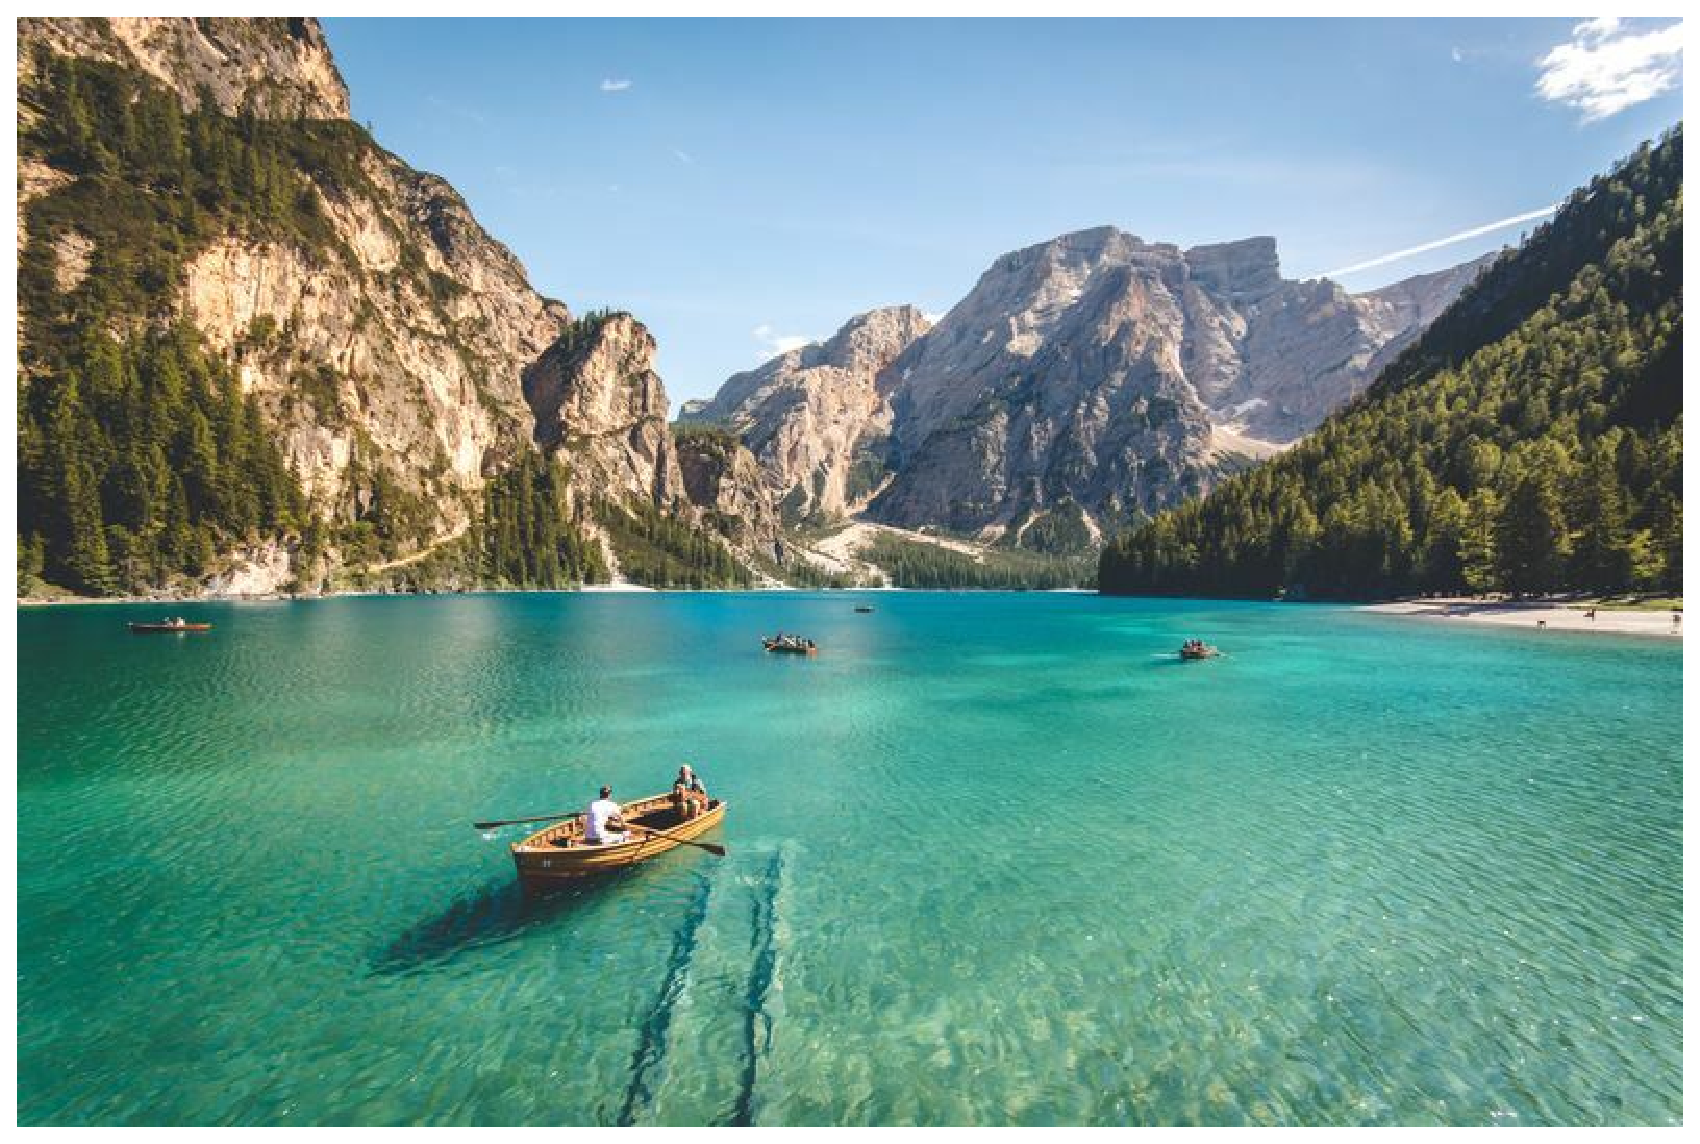
\includegraphics[height=50mm]{question_5/Image-1.eps} & 
			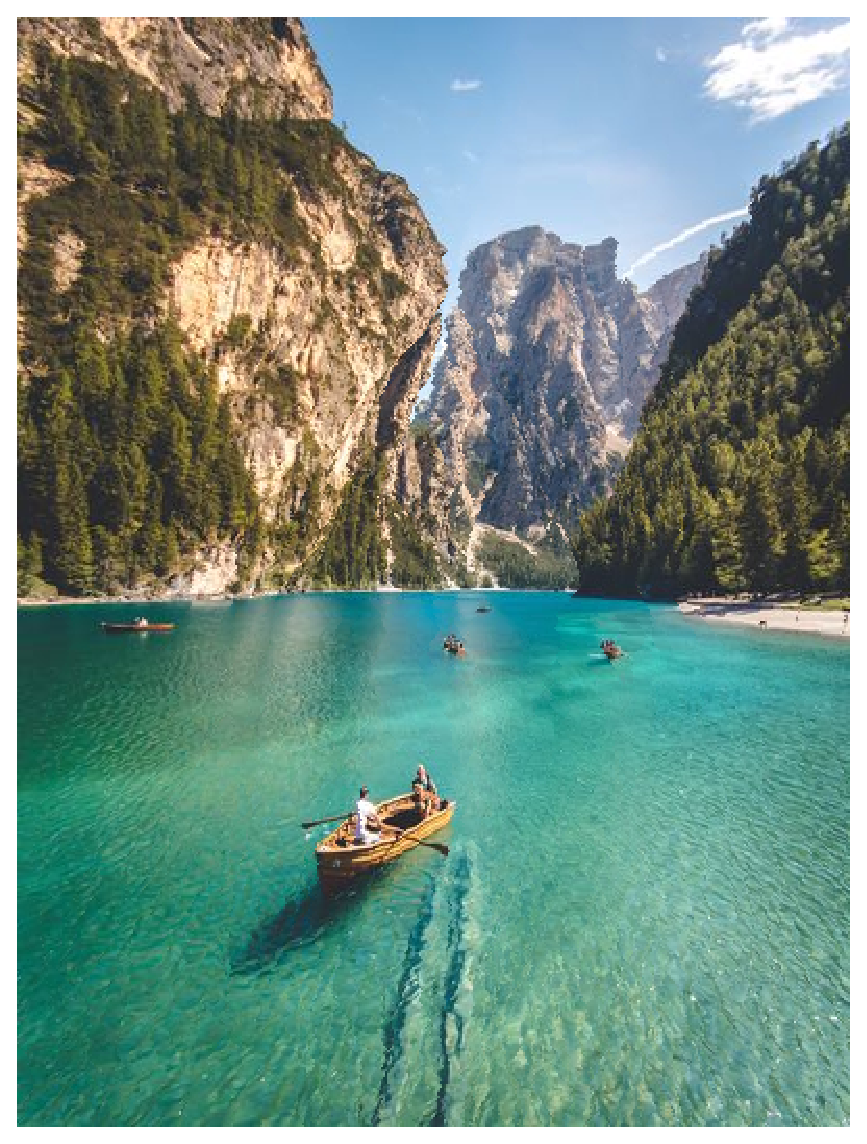
\includegraphics[height=50mm]{question_5/Image-1_scaled_column_by_0.5.eps} & 
				0.5 \\ \hline
			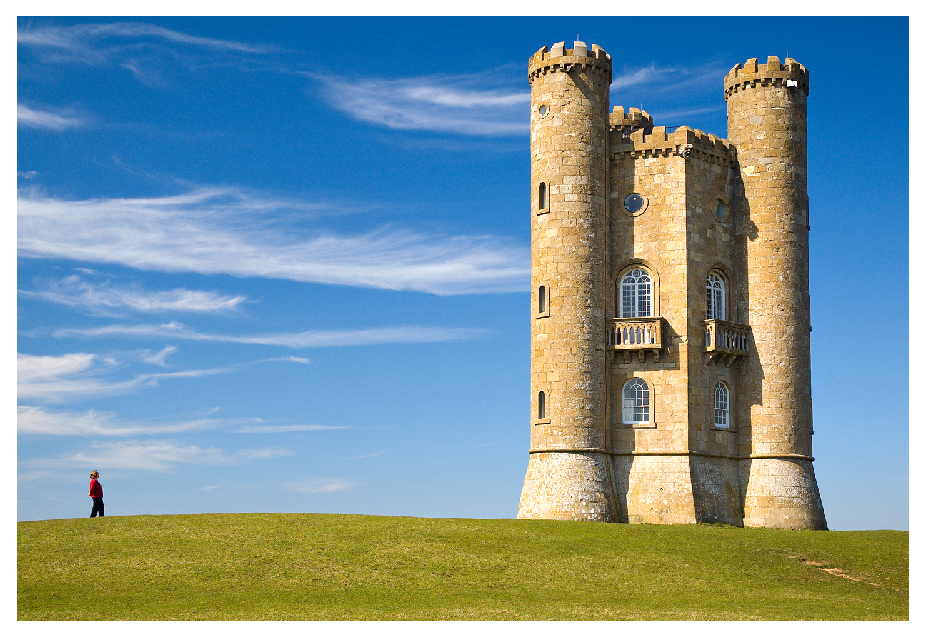
\includegraphics[height=50mm]{question_5/Image-2.eps} & 
			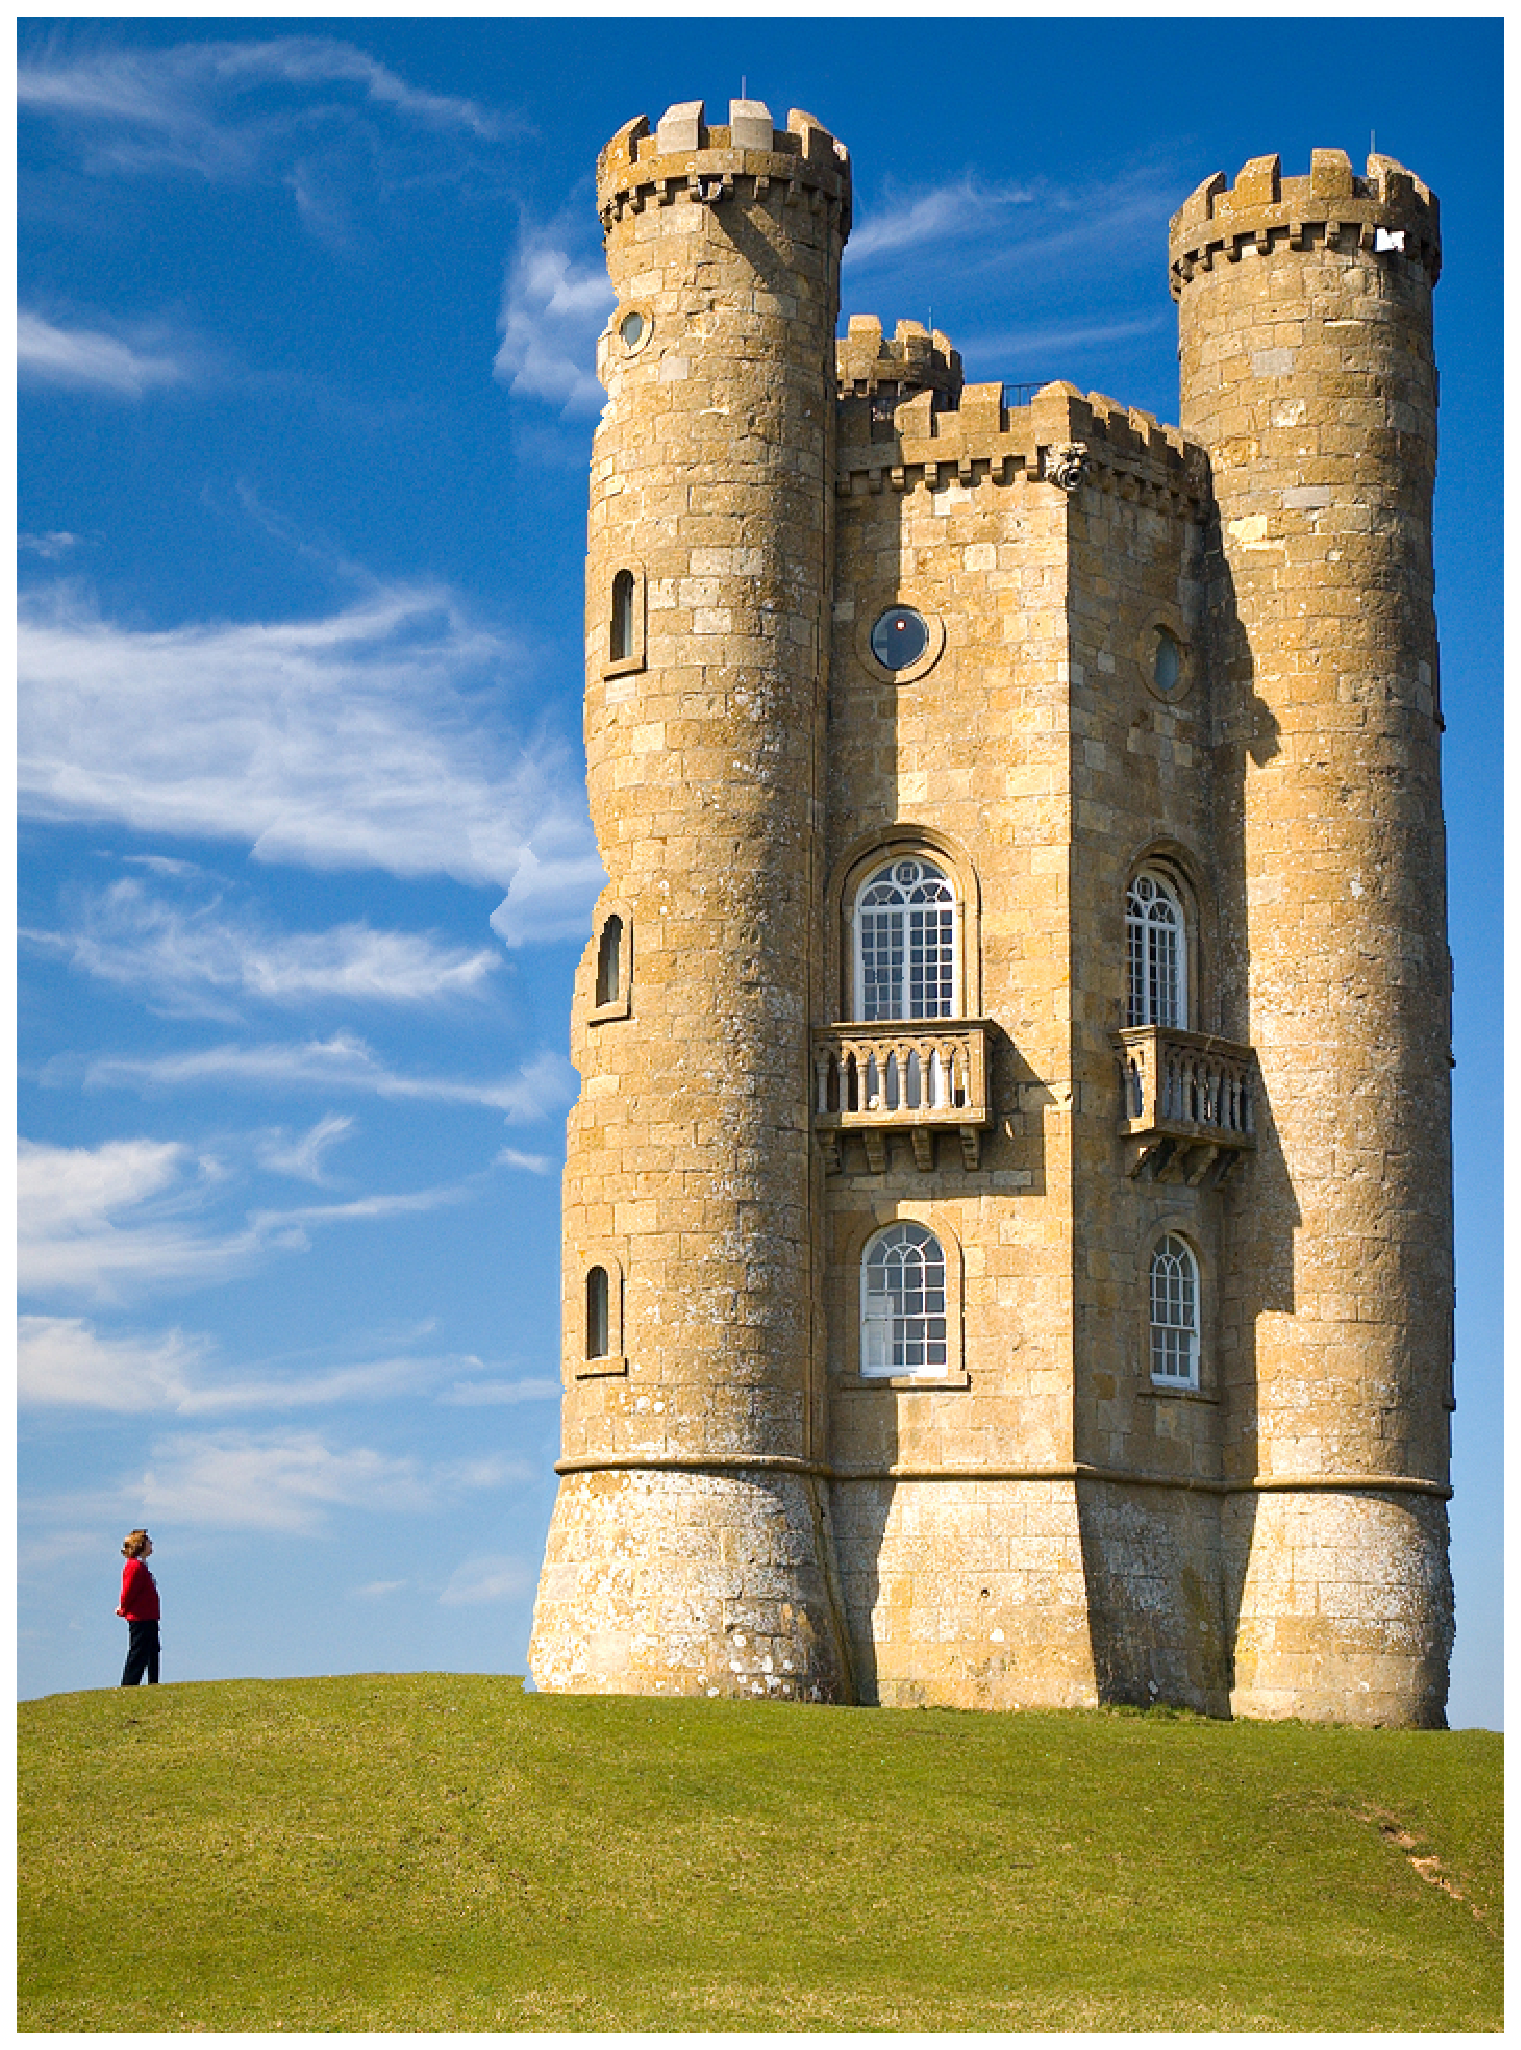
\includegraphics[height=50mm]{question_5/Image-2_scaled_column_by_0.5.eps} & 
				0.5 \\ \hline
		\end{tabular}
	\end{center}
\caption{Processed Images}
\end{table}

\clearpage
\section{Question 6}

\subsection{Task}
Consider a transformation by which a function $y_i\left(x_i\right)$ is transformed to another function $m_i\left(c_i\right)$  where $m$ and $c$ are slope and intercept of the original curve at different points on the curve represented by $y$ as function of $x$. The envelope of lines of slope $m$ drawn at each value of $c$ has the same shape as that of the curve drawn using the points $\left(x,y\right)$. This is illustrated a parabola as shown in the figures below. Write a program that converts a function given as $y\left(x\right)$ to the new form either graphically or analytically. Make sure your process works even when the function $y\left(x\right)$ is changed to any other smooth and well-behaved function.

\subsection{Solution}

Link to the GitHub repository for this question: \href{https://github.com/Xerefic/MM2090-Solutions/tree/master/Final_Assignment/question_6}{GitHub}

\subsubsection{Approach}
Sampling the given function for 50 points in the range $0 \leq x \leq 100$ and representing the said function using a scatter plot. The transformed function is nothing but the set of lines whose slope correspond to the slope of the tangent at a point $\left(x_i,y_i\right)$ on the polynomial. Using the derivative operation in sagemath, I am computing the slope at a point $x_i$ for $x_i \in f(x)$. At a point $x_i$, the modified function is given by $\frac{y-f(x_i)}{x-x_i}=\frac{\partial f(x)}{\partial x}_{x=x_i}$. 

\subsubsection{Requirements}
Language of choice: sagemath
\begin{lstlisting}[language=bash]
	pip3 install numpy
	pip3 install matplotlib
	pip3 install pandas
\end{lstlisting}

\subsubsection{Output}



\clearpage


\end{document}
